\chapter{Finding important/interesting stuff in the code}

Minimalism it is not a prominent feature of modern software.

\myindex{\Cpp!STL}

But not because the programmers are writing a lot, but because a lot of libraries are commonly linked statically
to executable files.
If all external libraries were shifted into an external DLL files, the world would be different.
(Another reason for C++ are the \ac{STL} and other template libraries.)

\newcommand{\FOOTNOTEBOOST}{\footnote{\url{http://www.boost.org/}}}
\newcommand{\FOOTNOTELIBPNG}{\footnote{\url{http://www.libpng.org/pub/png/libpng.html}}}

Thus, it is very important to determine the origin of a function, if it is from standard library or 
well-known library (like Boost\FOOTNOTEBOOST, libpng\FOOTNOTELIBPNG),
or if it is related to what we are trying to find in the code.

It is just absurd to rewrite all code in \CCpp to find what we're looking for.

One of the primary tasks of a reverse engineer is to find quickly the code he/she needs, and what is not that important.

\myindex{\GrepUsage}

The \IDA disassembler allow us to search among text strings, byte sequences and constants.
It is even possible to export the code to .lst or .asm text files and then use \TT{grep}, \TT{awk}, etc.

When you try to understand what some code is doing, this easily could be some open-source library like libpng.
So when you see some constants or text strings which look familiar, it is always worth to \emph{google} them.
And if you find the opensource project where they are used, 
then it's enough just to compare the functions.
It may solve some part of the problem.

For example, if a program uses XML files, the first step may be determining which
XML library is used for processing, since the standard (or well-known) libraries are usually used
instead of self-made one.

\myindex{SAP}
\myindex{Windows!PDB}

For example, the author of these lines once tried to understand how the compression/decompression of network packets works in SAP 6.0. 
It is a huge software, but a detailed .\gls{PDB} with debugging information is present, 
and that is convenient.
He finally came to the idea that one of the functions, that was called \emph{CsDecomprLZC}, was doing the decompression of network packets.
Immediately he tried to google its name and he quickly found the function was used in MaxDB
(it is an open-source SAP project) \footnote{More about it in relevant section~(\myref{sec:SAPGUI})}.

\url{http://www.google.com/search?q=CsDecomprLZC}

Astoundingly, MaxDB and SAP 6.0 software shared likewise code for the compression/decompression of network packets.

\mysection{Identification of executable files}

\subsection{Microsoft Visual C++}
\label{MSVC_versions}

MSVC versions and DLLs that can be imported:

%\small
\begin{center}
\begin{tabular}{ | l | l | l | l | l | }
\hline
\HeaderColor Marketing ver. & 
\HeaderColor Internal ver. & 
\HeaderColor CL.EXE ver. &
\HeaderColor DLLs imported &
\HeaderColor Release date \\
\hline
% 4.0, April 1995
% 97 & 5.0 & February 1997
6		&  6.0	& 12.00	& msvcrt.dll	& June 1998		\\
		&	&	& msvcp60.dll	&			\\
\hline
.NET (2002)	&  7.0	& 13.00	& msvcr70.dll	& February 13, 2002	\\
		&	&	& msvcp70.dll	&			\\
\hline
.NET 2003	&  7.1	& 13.10 & msvcr71.dll	& April 24, 2003	\\
		&	&	& msvcp71.dll	&			\\
\hline
2005		&  8.0	& 14.00 & msvcr80.dll	& November 7, 2005	\\
		&	&	& msvcp80.dll	&			\\
\hline
2008		&  9.0	& 15.00 & msvcr90.dll	& November 19, 2007	\\
		&	&	& msvcp90.dll	&			\\
\hline
2010		& 10.0	& 16.00 & msvcr100.dll	& April 12, 2010 	\\
		&	&	& msvcp100.dll	&			\\
\hline
2012		& 11.0	& 17.00 & msvcr110.dll	& September 12, 2012 	\\
		&	&	& msvcp110.dll	&			\\
\hline
2013		& 12.0	& 18.00 & msvcr120.dll	& October 17, 2013 	\\
		&	&	& msvcp120.dll	&			\\
\hline
\end{tabular}
\end{center}
%\normalsize

msvcp*.dll has \Cpp{}-related functions, so if it is imported, 
this is probably a \Cpp program.

\subsubsection{Name mangling}

The names usually start with the \TT{?} symbol.

You can read more about MSVC's \gls{name mangling} here: \myref{namemangling}.

\subsection{GCC}
\myindex{GCC}

Aside from *NIX targets, GCC is also present in the win32 environment, in the form of Cygwin and MinGW.

\subsubsection{Name mangling}

Names usually start with the \TT{\_Z} symbols.

You can read more about GCC's \gls{name mangling} here: \myref{namemangling}.

\subsubsection{Cygwin}
\myindex{Cygwin}

cygwin1.dll is often imported.

\subsubsection{MinGW}
\myindex{MinGW}

msvcrt.dll may be imported.

\subsection{Intel Fortran}
\myindex{Fortran}

libifcoremd.dll, libifportmd.dll and libiomp5md.dll (OpenMP support) may be imported.

libifcoremd.dll has a lot of functions prefixed with \TT{for\_}, which means \emph{Fortran}.

\subsection{Watcom, OpenWatcom}
\myindex{Watcom}
\myindex{OpenWatcom}

\subsubsection{Name mangling}

Names usually start with the \TT{W} symbol.

For example, that is how the method named \q{method} of the class \q{class} that does not have any arguments and returns
\Tvoid is encoded:

\begin{lstlisting}
W?method$_class$n__v
\end{lstlisting}

\subsection{Borland}
\myindex{Borland Delphi}
\myindex{Borland C++Builder}

Here is an example of Borland Delphi's and C++Builder's \gls{name mangling}:

\lstinputlisting{digging_into_code/identification/borland_mangling.txt}

The names always start with the \TT{@} 
symbol, then we have the class name came, method name, and encoded the types of the arguments of the method.

These names can be in the .exe imports, .dll exports, debug data, etc.

Borland Visual Component Libraries (VCL) 
are stored in .bpl files instead of .dll ones, for example, vcl50.dll, rtl60.dll.

Another DLL that might be imported: BORLNDMM.DLL.

\subsubsection{Delphi}

Almost all Delphi executables has the \q{Boolean} text string at the beginning of the code segment, along with other type names.

This is a very typical beginning of the \TT{CODE} 
segment of a Delphi program, this block came right after the win32 PE file header:

\lstinputlisting{digging_into_code/identification/delphi.txt}

The first 4 bytes of the data segment (\TT{DATA}) can be \TT{00 00 00 00}, \TT{32 13 8B C0} or \TT{FF FF FF FF}.%

This information can be useful when dealing with packed/encrypted Delphi executables.

\subsection{Other known DLLs}

\myindex{OpenMP}
\begin{itemize}
\item vcomp*.dll---Microsoft's implementation of OpenMP.
\end{itemize}



% binary files might be also here

\mysection{Communication with outer world (function level)}
It's often advisable to track function arguments and return values in debugger or \ac{DBI}.
For example, the author once tried to understand meaning of some obscure function, which happens to be incorrectly
implemented bubble sort\footnote{\url{https://yurichev.com/blog/weird_sort_KLEE/}}.
(It worked correctly, but slower.)
Meanwhile, watching inputs and outputs of this function helps instantly to understand what it does.

Often, when you see division by multiplication (\myref{sec:divisionbymult}),
but forgot all details about its mechanics, you can just observe input
and output and quickly find divisor.

% sections:
\mysection{Communication with the outer world (win32)}

Sometimes it's enough to observe some function's inputs and outputs in order to understand what it does.
That way you can save time.

Files and registry access: 
for the very basic analysis, Process Monitor\footnote{\url{http://technet.microsoft.com/en-us/sysinternals/bb896645.aspx}}
utility from SysInternals can help.

For the basic analysis of network accesses, Wireshark\footnote{\url{http://www.wireshark.org/}} can be useful.

But then you will have to look inside anyway. \\
\\
The first thing to look for is which functions from the \ac{OS}'s \ac{API}s and standard libraries are used.

If the program is divided into a main executable file and a group of DLL files, sometimes the names of the functions in these DLLs can help.

If we are interested in exactly what can lead to a call to \TT{MessageBox()} with specific text, 
we can try to find this text in the data segment, find the references to it and find the points
from which the control may be passed to the \TT{MessageBox()} call we're interested in.

\myindex{\CStandardLibrary!rand()}
If we are talking about a video game and we're interested in which events are more or less random in it,
we may try to find the \rand function or its replacements (like the Mersenne twister algorithm) and find the places
from which those functions are called, and more importantly, how are the results used.
% BUG in varioref: http://tex.stackexchange.com/questions/104261/varioref-vref-or-vpageref-at-page-boundary-may-loop
One example: \myref{chap:color_lines}. 

But if it is not a game, and \rand is still used, it is also interesting to know why.
There are cases of unexpected \rand usage in data compression algorithms (for encryption imitation):
\href{http://blog.yurichev.com/node/44}{blog.yurichev.com}.

\subsection{Often used functions in the Windows API}

These functions may be among the imported.
It is worth to note that not every function might be used in the code that was written by the programmer.
A lot of functions might be called from library functions and \ac{CRT} code.

Some functions may have the \GTT{-A} suffix for the ASCII version and \GTT{-W} for the Unicode version.

\begin{itemize}

\item
Registry access (advapi32.dll): 
RegEnumKeyEx, RegEnumValue, RegGetValue, RegOpenKeyEx, RegQueryValueEx.

\item
Access to text .ini-files (kernel32.dll): 
GetPrivateProfileString.

\item
Dialog boxes (user32.dll): 
MessageBox, MessageBoxEx, CreateDialog, SetDlgItemText, GetDlgItemText.

\item
Resources access (\myref{PEresources}): (user32.dll): LoadMenu.

\item
TCP/IP networking (ws2\_32.dll):
WSARecv, WSASend.

\item
File access (kernel32.dll):
CreateFile, ReadFile, ReadFileEx, WriteFile, WriteFileEx.

\item
High-level access to the Internet (wininet.dll): WinHttpOpen.

\item
Checking the digital signature of an executable file (wintrust.dll):
WinVerifyTrust.

\item
The standard MSVC library (if it's linked dynamically) (msvcr*.dll):
assert, itoa, ltoa, open, printf, read, strcmp, atol, atoi, fopen, fread, fwrite, memcmp, rand,
strlen, strstr, strchr.

\end{itemize}

\subsection{Extending trial period}

Registry access functions are frequent targets for those who try to crack trial period of some software, which may save
installation date/time into registry.

Another popular target are GetLocalTime() and GetSystemTime() functions:
a trial software, at each startup, must check current date/time somehow anyway.

\subsection{Removing nag dialog box}

A popular way to find out what causing popping nag dialog box is intercepting MessageBox(), 
CreateDialog() and CreateWindow() functions.

\subsection{tracer: Intercepting all functions in specific module}
\myindex{tracer}

\myindex{x86!\Instructions!INT3}
There are INT3 breakpoints in the \tracer, that are triggered only once, however, they can be set for all functions
in a specific DLL.

\begin{lstlisting}
--one-time-INT3-bp:somedll.dll!.*
\end{lstlisting}

Or, let's set INT3 breakpoints on all functions with the \TT{xml} prefix in their name:

\begin{lstlisting}
--one-time-INT3-bp:somedll.dll!xml.*
\end{lstlisting}

On the other side of the coin, such breakpoints are triggered only once.
Tracer will show the call of a function, if it happens, but only once.
Another drawback---it is impossible to see the function's arguments.

Nevertheless, this feature is very useful when you know that the program uses a DLL,
but you do not know which functions are actually used.
And there are a lot of functions. 

\par
\myindex{Cygwin}
For example, let's see, what does the uptime utility from cygwin use:

\begin{lstlisting}
tracer -l:uptime.exe --one-time-INT3-bp:cygwin1.dll!.*
\end{lstlisting}

Thus we may see all that cygwin1.dll library functions that were called at least once, and where from:

\lstinputlisting{digging_into_code/uptime_cygwin.txt}


\mysection{Strings}
\label{sec:digging_strings}

\mysection{Task manager practical joke (Windows Vista)}
\myindex{Windows!Windows Vista}

Let's see if it's possible to hack Task Manager slightly so it would detect more \ac{CPU} cores.

\myindex{Windows!NTAPI}

Let us first think, how does the Task Manager know the number of cores?

There is the \TT{GetSystemInfo()} win32 function present in win32 userspace which can tell us this.
But it's not imported in \TT{taskmgr.exe}.

There is, however, another one in \gls{NTAPI}, \TT{NtQuerySystemInformation()}, 
which is used in \TT{taskmgr.exe} in several places.

To get the number of cores, one has to call this function with the \TT{SystemBasicInformation} constant
as a first argument (which is zero
\footnote{\href{http://msdn.microsoft.com/en-us/library/windows/desktop/ms724509(v=vs.85).aspx}{MSDN}}).

The second argument has to point to the buffer which is getting all the information.

So we have to find all calls to the \\
\TT{NtQuerySystemInformation(0, ?, ?, ?)} function.
Let's open \TT{taskmgr.exe} in IDA. 
\myindex{Windows!PDB}

What is always good about Microsoft executables is that IDA can download the corresponding \gls{PDB} 
file for this executable and show all function names.

It is visible that Task Manager is written in \Cpp and some of the function names and classes are really 
speaking for themselves.
There are classes CAdapter, CNetPage, CPerfPage, CProcInfo, CProcPage, CSvcPage, 
CTaskPage, CUserPage.

Apparently, each class corresponds to each tab in Task Manager.

Let's visit each call and add comment with the value which is passed as the first function argument.
We will write \q{not zero} at some places, because the value there was clearly not zero, 
but something really different (more about this in the second part of this chapter).

And we are looking for zero passed as argument, after all.

\begin{figure}[H]
\centering
\myincludegraphics{examples/taskmgr/IDA_xrefs.png}
\caption{IDA: cross references to NtQuerySystemInformation()}
\end{figure}

Yes, the names are really speaking for themselves.

When we closely investigate each place where\\
\TT{NtQuerySystemInformation(0, ?, ?, ?)} is called,
we quickly find what we need in the \TT{InitPerfInfo()} function:

\lstinputlisting[caption=taskmgr.exe (Windows Vista),style=customasmx86]{examples/taskmgr/taskmgr.lst}

\TT{g\_cProcessors} is a global variable, and this name has been assigned by 
IDA according to the \gls{PDB} loaded from Microsoft's symbol server.

The byte is taken from \TT{var\_C20}. 
And \TT{var\_C58} is passed to\\
\TT{NtQuerySystemInformation()} 
as a pointer to the receiving buffer.
The difference between 0xC20 and 0xC58 is 0x38 (56).

Let's take a look at format of the return structure, which we can find in MSDN:

\begin{lstlisting}[style=customc]
typedef struct _SYSTEM_BASIC_INFORMATION {
    BYTE Reserved1[24];
    PVOID Reserved2[4];
    CCHAR NumberOfProcessors;
} SYSTEM_BASIC_INFORMATION;
\end{lstlisting}

This is a x64 system, so each PVOID takes 8 bytes.

All \emph{reserved} fields in the structure take $24+4*8=56$ bytes.

Oh yes, this implies that \TT{var\_C20} is the local stack is exactly the
\TT{NumberOfProcessors} field of the \TT{SYSTEM\_BASIC\_INFORMATION} structure.

Let's check our guess.
Copy \TT{taskmgr.exe} from \TT{C:\textbackslash{}Windows\textbackslash{}System32} 
to some other folder 
(so the \emph{Windows Resource Protection} 
will not try to restore the patched \TT{taskmgr.exe}).

Let's open it in Hiew and find the place:

\begin{figure}[H]
\centering
\myincludegraphics{examples/taskmgr/hiew2.png}
\caption{Hiew: find the place to be patched}
\end{figure}

Let's replace the \TT{MOVZX} instruction with ours.
Let's pretend we've got 64 CPU cores.

Add one additional \ac{NOP} (because our instruction is shorter than the original one):

\begin{figure}[H]
\centering
\myincludegraphics{examples/taskmgr/hiew1.png}
\caption{Hiew: patch it}
\end{figure}

And it works!
Of course, the data in the graphs is not correct.

At times, Task Manager even shows an overall CPU load of more than 100\%.

\begin{figure}[H]
\centering
\myincludegraphics{examples/taskmgr/taskmgr_64cpu_crop.png}
\caption{Fooled Windows Task Manager}
\end{figure}

The biggest number Task Manager does not crash with is 64.

Apparently, Task Manager in Windows Vista was not tested on computers with a large number of cores.

So there are probably some static data structure(s) inside it limited to 64 cores.

\subsection{Using LEA to load values}
\label{TaskMgr_LEA}

Sometimes, \TT{LEA} is used in \TT{taskmgr.exe} instead of \TT{MOV} to set the first argument of \\
\TT{NtQuerySystemInformation()}:

\lstinputlisting[caption=taskmgr.exe (Windows Vista),style=customasmx86]{examples/taskmgr/taskmgr2.lst}

\myindex{x86!\Instructions!LEA}

Perhaps \ac{MSVC} did so because machine code of \INS{LEA} is shorter than \INS{MOV REG, 5} (would be 5 instead of 4).

\INS{LEA} with offset in $-128..127$ range (offset will occupy 1 byte in opcode) with 32-bit registers is even shorter (for lack of REX prefix)---3 bytes.

Another example of such thing is: \myref{using_MOV_and_pack_of_LEA_to_load_values}.


\subsection{Finding strings in binary}

\epigraph{Actually, the best form of Unix documentation is frequently running the
\textbf{strings} command over a program’s object code. Using \textbf{strings}, you can get
a complete list of the program’s hard-coded file name, environment variables,
undocumented options, obscure error messages, and so forth.}{The Unix-Haters Handbook}

\myindex{UNIX!strings}
The standard UNIX \emph{strings} utility is quick-n-dirty way to see strings in file.
For example, these are some strings from OpenSSH 7.2 sshd executable file:

\lstinputlisting{digging_into_code/sshd_strings.txt}

There are options, error messages, file paths, imported dynamic modules and functions, some other strange strings (keys?)
There is also unreadable noise---x86 code sometimes has chunks consisting of printable ASCII characters, up to ~8 characters.

Of course, OpenSSH is open-source program.
But looking at readable strings inside of some unknown binary is often a first step of analysis.
\myindex{UNIX!grep}

\emph{grep} can be applied as well.

\myindex{Hiew}
\myindex{Sysinternals}
Hiew has the same capability (Alt-F6), as well as Sysinternals ProcessMonitor.

\subsection{Error/debug messages}

Debugging messages are very helpful if present.
In some sense, the debugging messages are reporting
what's going on in the program right now. Often these are \printf-like functions,
which write to log-files, or sometimes do not writing anything but the calls are still present 
since the build is not a debug one but \emph{release} one.
\myindex{\oracle}

If local or global variables are dumped in debug messages, it might be helpful as well 
since it is possible to get at least the variable names.
For example, one of such function in \oracle is \TT{ksdwrt()}.

Meaningful text strings are often helpful.
The \IDA disassembler may show from which function and from which point this specific string is used.
Funny cases sometimes happen\footnote{\href{http://blog.yurichev.com/node/32}{blog.yurichev.com}}.

The error messages may help us as well.
In \oracle, errors are reported using a group of functions.\\
You can read more about them here: \href{http://blog.yurichev.com/node/43}{blog.yurichev.com}.

\myindex{Error messages}

It is possible to find quickly which functions report errors and in which conditions.

By the way, this is often the reason why copy-protection systems use inarticulate cryptic error messages 
or just error numbers.
No software author is happy if the software cracker can quickly understands copy-protection's inner workings
judging by error messages it can produce.

One example of encrypted error messages is here: \myref{examples_SCO}.

\subsection{Suspicious magic strings}

Some magic strings which are usually used in backdoors look pretty suspicious.

For example, there was a backdoor in the TP-Link WR740 home router\footnote{\url{http://sekurak.pl/tp-link-httptftp-backdoor/}}.
The backdoor can activated using the following URL:\\
\url{http://192.168.0.1/userRpmNatDebugRpm26525557/start_art.html}.\\

Indeed, the \q{userRpmNatDebugRpm26525557} string is present in the firmware.

This string was not googleable until the wide disclosure of information about the backdoor.

You would not find this in any \ac{RFC}.

You would not find any computer science algorithm which uses such strange byte sequences.

And it doesn't look like an error or debugging message.

So it's a good idea to inspect the usage of such weird strings.\\
\\
\myindex{base64}

Sometimes, such strings are encoded using base64.

So it's a good idea to decode them all and to scan them visually, even a glance should be enough.\\
\\
\myindex{Security through obscurity}
More precise, this method of hiding backdoors is called \q{security through obscurity}.


\mysection{Calls to assert()}
\myindex{\CStandardLibrary!assert()}

Sometimes the presence of the \TT{assert()} macro is useful too: 
commonly this macro leaves source file name, line number and condition in the code.

The most useful information is contained in the assert's condition, we can deduce variable names or structure field
names from it. Another useful piece of information are the file names---we can try to deduce what type of
code is there.
Also it is possible to recognize well-known open-source libraries by the file names.

\lstinputlisting[caption=Example of informative assert() calls,style=customasmx86]{digging_into_code/assert_examples.lst}

It is advisable to \q{google} both the conditions and file names, which can lead us to an open-source library.
For example, if we \q{google} \q{sp->lzw\_nbits <= BITS\_MAX}, this predictably 
gives us some open-source code that's related to the LZW compression.

\mysection{Constants}

Humans, including programmers, often use round numbers like 10, 100, 1000, 
in real life as well as in the code.

The practicing reverse engineer usually know them well in hexadecimal representation:
10=0xA, 100=0x64, 1000=0x3E8, 10000=0x2710.

The constants \TT{0xAAAAAAAA} (0b10101010101010101010101010101010) and \\
\TT{0x55555555} (0b01010101010101010101010101010101)  are also popular---those
are composed of alternating bits.

That may help to distinguish some signal from a signal where all bits are turned on (0b1111 \dots) or off (0b0000 \dots).
For example, the \TT{0x55AA} constant
is used at least in the boot sector, \ac{MBR}, 
and in the \ac{ROM} of IBM-compatible extension cards.

Some algorithms, especially cryptographical ones use distinct constants, which are easy to find
in code using \IDA.

\myindex{MD5}

For example, the MD5 algorithm initializes its own internal variables like this:

\begin{verbatim}
var int h0 := 0x67452301
var int h1 := 0xEFCDAB89
var int h2 := 0x98BADCFE
var int h3 := 0x10325476
\end{verbatim}

If you find these four constants used in the code in a row, it is highly probable that this function is related to MD5.

\par Another example are the CRC16/CRC32 algorithms, 
whose calculation algorithms often use precomputed tables like this one:

\begin{lstlisting}[caption=linux/lib/crc16.c,style=customc]
/** CRC table for the CRC-16. The poly is 0x8005 (x^16 + x^15 + x^2 + 1) */
u16 const crc16_table[256] = {
	0x0000, 0xC0C1, 0xC181, 0x0140, 0xC301, 0x03C0, 0x0280, 0xC241,
	0xC601, 0x06C0, 0x0780, 0xC741, 0x0500, 0xC5C1, 0xC481, 0x0440,
	0xCC01, 0x0CC0, 0x0D80, 0xCD41, 0x0F00, 0xCFC1, 0xCE81, 0x0E40,
	...
\end{lstlisting}

See also the precomputed table for CRC32: \myref{sec:CRC32}.

In tableless CRC algorithms well-known polynomials are used, for example, 0xEDB88320 for CRC32.

\subsection{Magic numbers}
\label{magic_numbers}

A lot of file formats define a standard file header where a \emph{magic number(s)} is used, single one or even several.

\myindex{MS-DOS}

For example, all Win32 and MS-DOS executables start with the two characters \q{MZ}.

\myindex{MIDI}

At the beginning of a MIDI file the \q{MThd} signature must be present. 
If we have a program which uses MIDI files for something,
it's very likely that it must check the file for validity by checking at least the first 4 bytes.

This could be done like this:
(\emph{buf} points to the beginning of the loaded file in memory)

\begin{lstlisting}[style=customasmx86]
cmp [buf], 0x6468544D ; "MThd"
jnz _error_not_a_MIDI_file
\end{lstlisting}

\myindex{\CStandardLibrary!memcmp()}
\myindex{x86!\Instructions!CMPSB}

\dots or by calling a function for comparing memory blocks like \TT{memcmp()} or any other equivalent code
up to a \TT{CMPSB} (\myref{REPE_CMPSx}) instruction.

When you find such point you already can say where the loading of the MIDI file starts,
also, we could see the location
of the buffer with the contents of the MIDI file, what is used from the buffer, and how.

\subsubsection{Dates}

\myindex{UFS2}
\myindex{FreeBSD}
\myindex{HASP}

Often, one may encounter number like \TT{0x19870116}, which is clearly looks like a date (year 1987, 1th month (January), 16th day).
This may be someone's birthday date (a programmer, his/her relative, child), or some other important date.
The date may also be written in a reverse order, like \TT{0x16011987}.
American-style dates are also popular, like \TT{0x01161987}.

Well-known example is \TT{0x19540119} (magic number used in UFS2 superblock structure), which is a birthday date of Marshall Kirk McKusick, prominent FreeBSD contributor.

\myindex{Stuxnet}
Stuxnet uses the number ``19790509'' (not as 32-bit number, but as string, though), and this led to speculation
that the malware is connected to Israel%
\footnote{This is a date of execution of Habib Elghanian, persian jew.}.

Also, numbers like those are very popular in amateur-grade cryptography, for example, excerpt from the \emph{secret function} internals from HASP3 dongle
\footnote{\url{https://web.archive.org/web/20160311231616/http://www.woodmann.com/fravia/bayu3.htm}}:

\begin{lstlisting}[style=customc]
void xor_pwd(void) 
{ 
	int i; 
	
	pwd^=0x09071966;
	for(i=0;i<8;i++) 
	{ 
		al_buf[i]= pwd & 7; pwd = pwd >> 3; 
	} 
};

void emulate_func2(unsigned short seed)
{ 
	int i, j; 
	for(i=0;i<8;i++) 
	{ 
		ch[i] = 0; 
		
		for(j=0;j<8;j++)
		{ 
			seed *= 0x1989; 
			seed += 5; 
			ch[i] |= (tab[(seed>>9)&0x3f]) << (7-j); 
		}
	} 
}
\end{lstlisting}

\subsubsection{DHCP}

This applies to network protocols as well.
For example, the DHCP protocol's network packets contains the so-called \emph{magic cookie}: \TT{0x63538263}.
Any code that generates DHCP packets somewhere must embed this constant into the packet.
If we find it in the code we may find where this happens and, not only that.
Any program which can receive DHCP packet must verify the \emph{magic cookie}, comparing it with the constant.

For example, let's take the dhcpcore.dll file from Windows 7 x64 and search for the constant.
And we can find it, twice:
it seems that the constant is used in two functions with descriptive names\\
\TT{DhcpExtractOptionsForValidation()} and \TT{DhcpExtractFullOptions()}:

\begin{lstlisting}[caption=dhcpcore.dll (Windows 7 x64),style=customasmx86]
.rdata:000007FF6483CBE8 dword_7FF6483CBE8 dd 63538263h          ; DATA XREF: DhcpExtractOptionsForValidation+79
.rdata:000007FF6483CBEC dword_7FF6483CBEC dd 63538263h          ; DATA XREF: DhcpExtractFullOptions+97
\end{lstlisting}

And here are the places where these constants are accessed:

\begin{lstlisting}[caption=dhcpcore.dll (Windows 7 x64),style=customasmx86]
.text:000007FF6480875F  mov     eax, [rsi]
.text:000007FF64808761  cmp     eax, cs:dword_7FF6483CBE8
.text:000007FF64808767  jnz     loc_7FF64817179
\end{lstlisting}

And:

\begin{lstlisting}[caption=dhcpcore.dll (Windows 7 x64),style=customasmx86]
.text:000007FF648082C7  mov     eax, [r12]
.text:000007FF648082CB  cmp     eax, cs:dword_7FF6483CBEC
.text:000007FF648082D1  jnz     loc_7FF648173AF
\end{lstlisting}

\subsection{Specific constants}

Sometimes, there is a specific constant for some type of code.
For example, the author once dug into a code, where number 12 was encountered suspiciously often.
Size of many arrays is 12, or multiple of 12 (24, etc).
As it turned out, that code takes 12-channel audio file at input and process it.

And vice versa: for example, if a program works with text field which has length of 120 bytes,
there has to be a constant 120 or 119 somewhere in the code.
If UTF-16 is used, then $2 \cdot 120$.
If a code works with network packets of fixed size, it's good idea to search for this constant in the code as well.

This is also true for amateur cryptography (license keys, etc).
If encrypted block has size of $n$ bytes, you may want to try to find occurences of this number throughout the code.
Also, if you see a piece of code which is been repeated $n$ times in loop during execution,
this may be encryption/decryption routine.

\subsection{Searching for constants}

It is easy in \IDA: Alt-B or Alt-I.
\myindex{binary grep}
And for searching for a constant in a big pile of files, or for searching in non-executable files,
there is a small utility called \emph{binary grep}\footnote{\BGREPURL}.


\mysection{Finding the right instructions}

If the program is utilizing FPU instructions and there are very few of them in the code,
one can try to check each one manually with a debugger.

\par For example, we may be interested how Microsoft Excel calculates the formulae entered by user.
For example, the division operation.

\myindex{\GrepUsage}
\myindex{x86!\Instructions!FDIV}

If we load excel.exe (from Office 2010) version 14.0.4756.1000 into \IDA, make a full listing
and to find every \FDIV instruction (except the ones which use constants as a second 
operand---obviously, they do not suit us):

\begin{lstlisting}
cat EXCEL.lst | grep fdiv | grep -v dbl_ > EXCEL.fdiv
\end{lstlisting}

\dots then we see that there are 144 of them.

\par We can enter a string like \TT{=(1/3)} in Excel and check each instruction.

\myindex{tracer}

\par By checking each instruction in a debugger or \tracer
(one may check 4 instruction at a time),
we get lucky and the sought-for instruction is just the 14th:

\begin{lstlisting}[style=customasmx86]
.text:3011E919 DC 33          fdiv    qword ptr [ebx]
\end{lstlisting}

\begin{lstlisting}
PID=13944|TID=28744|(0) 0x2f64e919 (Excel.exe!BASE+0x11e919)
EAX=0x02088006 EBX=0x02088018 ECX=0x00000001 EDX=0x00000001
ESI=0x02088000 EDI=0x00544804 EBP=0x0274FA3C ESP=0x0274F9F8
EIP=0x2F64E919
FLAGS=PF IF
FPU ControlWord=IC RC=NEAR PC=64bits PM UM OM ZM DM IM 
FPU StatusWord=
FPU ST(0): 1.000000
\end{lstlisting}

\ST{0} holds the first argument (1) and second one is in \TT{[EBX]}.\\
\\
\myindex{x86!\Instructions!FDIV}

The instruction after \FDIV (\TT{FSTP}) writes the result in memory:\\

\begin{lstlisting}[style=customasmx86]
.text:3011E91B DD 1E          fstp    qword ptr [esi]
\end{lstlisting}

If we set a breakpoint on it, we can see the result:

\begin{lstlisting}
PID=32852|TID=36488|(0) 0x2f40e91b (Excel.exe!BASE+0x11e91b)
EAX=0x00598006 EBX=0x00598018 ECX=0x00000001 EDX=0x00000001
ESI=0x00598000 EDI=0x00294804 EBP=0x026CF93C ESP=0x026CF8F8
EIP=0x2F40E91B
FLAGS=PF IF
FPU ControlWord=IC RC=NEAR PC=64bits PM UM OM ZM DM IM 
FPU StatusWord=C1 P 
FPU ST(0): 0.333333
\end{lstlisting}

Also as a practical joke, we can modify it on the fly:

\begin{lstlisting}
tracer -l:excel.exe bpx=excel.exe!BASE+0x11E91B,set(st0,666)
\end{lstlisting}

\begin{lstlisting}
PID=36540|TID=24056|(0) 0x2f40e91b (Excel.exe!BASE+0x11e91b)
EAX=0x00680006 EBX=0x00680018 ECX=0x00000001 EDX=0x00000001
ESI=0x00680000 EDI=0x00395404 EBP=0x0290FD9C ESP=0x0290FD58
EIP=0x2F40E91B
FLAGS=PF IF
FPU ControlWord=IC RC=NEAR PC=64bits PM UM OM ZM DM IM 
FPU StatusWord=C1 P 
FPU ST(0): 0.333333
Set ST0 register to 666.000000
\end{lstlisting}

Excel shows 666 in the cell, finally convincing us that we have found the right point.

\begin{figure}[H]
\centering
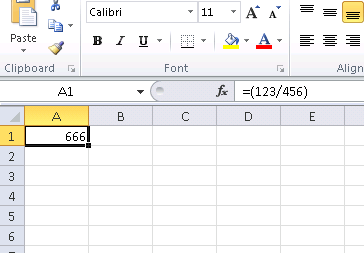
\includegraphics[width=0.6\textwidth]{digging_into_code/Excel_prank.png}
\caption{The practical joke worked}
\end{figure}

If we try the same Excel version, but in x64,
we will find only 12 \FDIV instructions there,
and the one we looking for is the third one.

\begin{lstlisting}
tracer.exe -l:excel.exe bpx=excel.exe!BASE+0x1B7FCC,set(st0,666)
\end{lstlisting}

\myindex{x86!\Instructions!DIVSD}

It seems that a lot of division operations of \Tfloat and \Tdouble types, were replaced by the compiler with SSE instructions
like \TT{DIVSD} (\TT{DIVSD} is present 268 times in total).

\mysection{Suspicious code patterns}

\subsection{XOR instructions}
\myindex{x86!\Instructions!XOR}

Instructions like \TT{XOR op, op} (for example, \TT{XOR EAX, EAX}) 
are usually used for setting the register value
to zero, but if the operands are different, the \q{exclusive or} operation
is executed.

This operation is rare in common programming, but widespread in cryptography,
including amateur one.
It's especially suspicious if the
second operand is a big number.

This may point to encrypting/decrypting, checksum computing, etc.\\
\\

One exception to this observation worth noting is the \q{canary} (\myref{subsec:BO_protection}). 
Its generation and checking are often done using the \XOR instruction. \\
\\
\myindex{AWK}

This AWK script can be used for processing \IDA{} listing (.lst) files:

\lstinputlisting{digging_into_code/awk.sh}

It is also worth noting that this kind of script can also match incorrectly disassembled code 
(\myref{sec:incorrectly_disasmed_code}).

\subsection{Hand-written assembly code}

\myindex{Function prologue}
\myindex{Function epilogue}
\myindex{x86!\Instructions!LOOP}
\myindex{x86!\Instructions!RCL}

Modern compilers do not emit the \TT{LOOP} and \TT{RCL} instructions.
On the other hand, these instructions are well-known to coders who like to code directly in assembly language.
If you spot these, it can be said that there is a high probability that this fragment of code was hand-written.
Such instructions are marked as (M) in the instructions list in this appendix: \myref{sec:x86_instructions}.

\par
Also the function prologue/epilogue are not commonly present in hand-written assembly.

\par
Commonly there is no fixed system for passing arguments to functions in the hand-written code.

\par
Example from the Windows 2003 kernel 
(ntoskrnl.exe file):

\lstinputlisting[style=customasmx86]{digging_into_code/ntoskrnl.lst}

Indeed, if we look in the 
\ac{WRK} v1.2 source code, this code
can be found easily in file \\
\emph{WRK-v1.2\textbackslash{}base\textbackslash{}ntos\textbackslash{}ke\textbackslash{}i386\textbackslash{}cpu.asm}.

\par 
As of \INS{RCL} instruction, I can find it in the ntoskrnl.exe file in Windows 2003 x86 (compiled with MS Visual C compiler).
It is occurred only once there, \\
in \TT{RtlExtendedLargeIntegerDivide()} function, and this might be inline assembler code case.


\mysection{Using magic numbers while tracing}

Often, our main goal is to understand how the program uses a value that has been either read from file or received via network. 
The manual tracing of a value is often a very labor-intensive task. One of the simplest techniques for this (although not 100\% reliable) 
is to use your own \emph{magic number}.

This resembles X-ray computed tomography is some sense: a radiocontrast agent is injected into the patient's blood,
which is then used to improve the visibility of the patient's internal structure in to the X-rays.
It is well known how the blood of healthy humans
percolates in the kidneys and if the agent is in the blood, it can be easily seen on tomography, how blood is percolating,
and are there any stones or tumors.

We can take a 32-bit number like \TT{0x0badf00d}, or someone's birth date like \TT{0x11101979}
and write this 4-byte number to some point in a file used by the program we investigate.

\myindex{\GrepUsage}
\myindex{tracer}

Then, while tracing this program with \tracer in \emph{code coverage} mode, with the help of \emph{grep}
or just by searching in the text file (of tracing results), we can easily see where the value has been used and how.

Example 
of \emph{grepable} \tracer results in \emph{cc} mode:

\begin{lstlisting}[style=customasmx86]
0x150bf66 (_kziaia+0x14), e=       1 [MOV EBX, [EBP+8]] [EBP+8]=0xf59c934 
0x150bf69 (_kziaia+0x17), e=       1 [MOV EDX, [69AEB08h]] [69AEB08h]=0 
0x150bf6f (_kziaia+0x1d), e=       1 [FS: MOV EAX, [2Ch]] 
0x150bf75 (_kziaia+0x23), e=       1 [MOV ECX, [EAX+EDX*4]] [EAX+EDX*4]=0xf1ac360 
0x150bf78 (_kziaia+0x26), e=       1 [MOV [EBP-4], ECX] ECX=0xf1ac360 
\end{lstlisting}
% TODO: good example!

This can be used for network packets as well.
It is important for the \emph{magic number} to be unique and not to be present in the program's code.

\newcommand{\DOSBOXURL}{\href{http://blog.yurichev.com/node/55}{blog.yurichev.com}}

\myindex{DosBox}
\myindex{MS-DOS}
Aside of 
the \tracer, DosBox (MS-DOS emulator) in heavydebug mode
is able to write information about all registers' states for each executed instruction of the program to a plain text file\footnote{See also my 
blog post about this DosBox feature: \DOSBOXURL{}}, so this technique may be useful for DOS programs as well.


\mysection{Loops}

Whenever your program works with some kind of file, or buffer of some size,
it has to be some kind of decrypting/processing loop inside of the code.

This is a real example of \tracer tool output.
There was a code which loads some kind of encryted file of 258 bytes.
I run it with the intention to get each instruction counts (a \ac{DBI} tool will serve much better these days).
And I quickly found a piece of code, which executed 259/258 times:

\lstinputlisting{digging_into_code/crypto_loop.txt}

As it turns out, this is the decrypting loop.


\mysection{Task manager practical joke (Windows Vista)}
\myindex{Windows!Windows Vista}

Let's see if it's possible to hack Task Manager slightly so it would detect more \ac{CPU} cores.

\myindex{Windows!NTAPI}

Let us first think, how does the Task Manager know the number of cores?

There is the \TT{GetSystemInfo()} win32 function present in win32 userspace which can tell us this.
But it's not imported in \TT{taskmgr.exe}.

There is, however, another one in \gls{NTAPI}, \TT{NtQuerySystemInformation()}, 
which is used in \TT{taskmgr.exe} in several places.

To get the number of cores, one has to call this function with the \TT{SystemBasicInformation} constant
as a first argument (which is zero
\footnote{\href{http://msdn.microsoft.com/en-us/library/windows/desktop/ms724509(v=vs.85).aspx}{MSDN}}).

The second argument has to point to the buffer which is getting all the information.

So we have to find all calls to the \\
\TT{NtQuerySystemInformation(0, ?, ?, ?)} function.
Let's open \TT{taskmgr.exe} in IDA. 
\myindex{Windows!PDB}

What is always good about Microsoft executables is that IDA can download the corresponding \gls{PDB} 
file for this executable and show all function names.

It is visible that Task Manager is written in \Cpp and some of the function names and classes are really 
speaking for themselves.
There are classes CAdapter, CNetPage, CPerfPage, CProcInfo, CProcPage, CSvcPage, 
CTaskPage, CUserPage.

Apparently, each class corresponds to each tab in Task Manager.

Let's visit each call and add comment with the value which is passed as the first function argument.
We will write \q{not zero} at some places, because the value there was clearly not zero, 
but something really different (more about this in the second part of this chapter).

And we are looking for zero passed as argument, after all.

\begin{figure}[H]
\centering
\myincludegraphics{examples/taskmgr/IDA_xrefs.png}
\caption{IDA: cross references to NtQuerySystemInformation()}
\end{figure}

Yes, the names are really speaking for themselves.

When we closely investigate each place where\\
\TT{NtQuerySystemInformation(0, ?, ?, ?)} is called,
we quickly find what we need in the \TT{InitPerfInfo()} function:

\lstinputlisting[caption=taskmgr.exe (Windows Vista),style=customasmx86]{examples/taskmgr/taskmgr.lst}

\TT{g\_cProcessors} is a global variable, and this name has been assigned by 
IDA according to the \gls{PDB} loaded from Microsoft's symbol server.

The byte is taken from \TT{var\_C20}. 
And \TT{var\_C58} is passed to\\
\TT{NtQuerySystemInformation()} 
as a pointer to the receiving buffer.
The difference between 0xC20 and 0xC58 is 0x38 (56).

Let's take a look at format of the return structure, which we can find in MSDN:

\begin{lstlisting}[style=customc]
typedef struct _SYSTEM_BASIC_INFORMATION {
    BYTE Reserved1[24];
    PVOID Reserved2[4];
    CCHAR NumberOfProcessors;
} SYSTEM_BASIC_INFORMATION;
\end{lstlisting}

This is a x64 system, so each PVOID takes 8 bytes.

All \emph{reserved} fields in the structure take $24+4*8=56$ bytes.

Oh yes, this implies that \TT{var\_C20} is the local stack is exactly the
\TT{NumberOfProcessors} field of the \TT{SYSTEM\_BASIC\_INFORMATION} structure.

Let's check our guess.
Copy \TT{taskmgr.exe} from \TT{C:\textbackslash{}Windows\textbackslash{}System32} 
to some other folder 
(so the \emph{Windows Resource Protection} 
will not try to restore the patched \TT{taskmgr.exe}).

Let's open it in Hiew and find the place:

\begin{figure}[H]
\centering
\myincludegraphics{examples/taskmgr/hiew2.png}
\caption{Hiew: find the place to be patched}
\end{figure}

Let's replace the \TT{MOVZX} instruction with ours.
Let's pretend we've got 64 CPU cores.

Add one additional \ac{NOP} (because our instruction is shorter than the original one):

\begin{figure}[H]
\centering
\myincludegraphics{examples/taskmgr/hiew1.png}
\caption{Hiew: patch it}
\end{figure}

And it works!
Of course, the data in the graphs is not correct.

At times, Task Manager even shows an overall CPU load of more than 100\%.

\begin{figure}[H]
\centering
\myincludegraphics{examples/taskmgr/taskmgr_64cpu_crop.png}
\caption{Fooled Windows Task Manager}
\end{figure}

The biggest number Task Manager does not crash with is 64.

Apparently, Task Manager in Windows Vista was not tested on computers with a large number of cores.

So there are probably some static data structure(s) inside it limited to 64 cores.

\subsection{Using LEA to load values}
\label{TaskMgr_LEA}

Sometimes, \TT{LEA} is used in \TT{taskmgr.exe} instead of \TT{MOV} to set the first argument of \\
\TT{NtQuerySystemInformation()}:

\lstinputlisting[caption=taskmgr.exe (Windows Vista),style=customasmx86]{examples/taskmgr/taskmgr2.lst}

\myindex{x86!\Instructions!LEA}

Perhaps \ac{MSVC} did so because machine code of \INS{LEA} is shorter than \INS{MOV REG, 5} (would be 5 instead of 4).

\INS{LEA} with offset in $-128..127$ range (offset will occupy 1 byte in opcode) with 32-bit registers is even shorter (for lack of REX prefix)---3 bytes.

Another example of such thing is: \myref{using_MOV_and_pack_of_LEA_to_load_values}.

% FIXME comparison!
\subsection{Memory \q{snapshots} comparing}
\label{snapshots_comparing}

The technique of the straightforward comparison of two memory snapshots in order to see changes was often used to hack
8-bit computer games and for hacking \q{high score} files.

For example, if you had a loaded game on an 8-bit computer (there isn't much memory on these, but the game usually
consumes even less memory) and you know that you have now, let's say, 100 bullets, you can do a \q{snapshot}
of all memory and back it up to some place. Then shoot once, the bullet count goes to 99, do a second \q{snapshot}
and then compare both: it must be a byte somewhere which has been 100 at the beginning, and now it is 99.

Considering the fact that these 8-bit games were often written in assembly language and such variables were global,
it can be said for sure which address in memory has holding the bullet count. If you searched for all references to the
address in the disassembled game code, it was not very hard to find a piece of code \glslink{decrement}{decrementing} the bullet count,
then to write a \gls{NOP} instruction there, or a couple of \gls{NOP}-s, 
and then have a game with 100 bullets forever.
\myindex{BASIC!POKE}
Games on these 8-bit computers were commonly loaded at the constant
address, also, there were not much different versions of each game (commonly just one version was popular for a long span of time),
so enthusiastic gamers knew which bytes must be overwritten (using the BASIC's instruction \gls{POKE}) at which address in
order to hack it. This led to \q{cheat} lists that contained \gls{POKE} instructions, published in magazines related to
8-bit games.

\myindex{MS-DOS}

Likewise, it is easy to modify \q{high score} files, this does not work with just 8-bit games. Notice 
your score count and back up the file somewhere. When the \q{high score} count gets different, just compare the two files,
it can even be done with the DOS utility FC\footnote{MS-DOS utility for comparing binary files} (\q{high score} files
are often in binary form).

There will be a point where a couple of bytes are different and it is easy to see which ones are
holding the score number.
However, game developers are fully aware of such tricks and may defend the program against it.

Somewhat similar example in this book is: \myref{Millenium_DOS_game}.

% TODO: пример с какой-то простой игрушкой?

\subsubsection{A real story from 1999}

\myindex{ICQ}
There was a time of ICQ messenger's popularity, at least in ex-USSR countries.
The messenger had a peculiarity --- some users didn't want to share their online status with everyone.
And you had to ask an \emph{authorization} from that user.
That user could allow you seeing his/her status, or maybe not.

This is what the author of these lines did:

\begin{itemize}
\item Added a user.
\item A user appeared in a contact-list, in a ``wait for authorization'' section.
\item Closed ICQ.
\item Backed up the ICQ database.
\item Loaded ICQ again.
\item User \emph{authorized}.
\item Closed ICQ and compared two databases.
\end{itemize}

It turned out: two database differed by only one byte.
In the first version: \verb|RESU\x03|, in the second: \verb|RESU\x02|.
(``RESU'', presumably, means ``USER'', i.e., a header of a structure where all the information about user was stored.)
That means the information about authorization was stored not at the server, but at the client.
Presumably, 2/3 value reflected \emph{authorization} status.

\subsubsection{Windows registry}

It is also possible to compare the Windows registry before and after a program installation.

It is a very popular method of finding which registry elements are used by the program.
Perhaps, this is the reason why the \q{windows registry cleaner} shareware is so popular.

By the way, this is how to dump Windows registry to text files:

\begin{lstlisting}
reg export HKLM HKLM.reg
reg export HKCU HKCU.reg
reg export HKCR HKCR.reg
reg export HKU HKU.reg
reg export HKCC HKCC.reg
\end{lstlisting}

\myindex{UNIX!diff}
They can be compared using diff...

\subsubsection{Engineering software, CADs, etc}

If a software uses proprietary files, you can also investigate something here as well.
You save file.
Then you add a dot or line or another primitive.
Save file, compare.
Or move dot, save file, compare.

\subsubsection{Blink-comparator}

Comparison of files or memory snapshots remind us blink-comparator
\footnote{\url{https://en.wikipedia.org/wiki/Blink_comparator}}:
a device used by astronomers in past, intended to find moving celestial objects.

Blink-comparator allows to switch quickly between two photographies shot in different time,
so astronomer would spot the difference visually.

By the way, Pluto was discovered by blink-comparator in 1930.

\mysection{\ac{ISA} detection}
\label{ISA_detect}

Often, you can deal with a binary file for an unknown \ac{ISA}.
Perhaps, easiest way to detect \ac{ISA} is to try various ones in IDA, objdump or another disassembler.

To achieve this, one should understand a difference between incorrectly disassembled code and correctly one.

% subsection:
\renewcommand{\CURPATH}{digging_into_code/incorrect_disassembly}
\mysection{Task manager practical joke (Windows Vista)}
\myindex{Windows!Windows Vista}

Let's see if it's possible to hack Task Manager slightly so it would detect more \ac{CPU} cores.

\myindex{Windows!NTAPI}

Let us first think, how does the Task Manager know the number of cores?

There is the \TT{GetSystemInfo()} win32 function present in win32 userspace which can tell us this.
But it's not imported in \TT{taskmgr.exe}.

There is, however, another one in \gls{NTAPI}, \TT{NtQuerySystemInformation()}, 
which is used in \TT{taskmgr.exe} in several places.

To get the number of cores, one has to call this function with the \TT{SystemBasicInformation} constant
as a first argument (which is zero
\footnote{\href{http://msdn.microsoft.com/en-us/library/windows/desktop/ms724509(v=vs.85).aspx}{MSDN}}).

The second argument has to point to the buffer which is getting all the information.

So we have to find all calls to the \\
\TT{NtQuerySystemInformation(0, ?, ?, ?)} function.
Let's open \TT{taskmgr.exe} in IDA. 
\myindex{Windows!PDB}

What is always good about Microsoft executables is that IDA can download the corresponding \gls{PDB} 
file for this executable and show all function names.

It is visible that Task Manager is written in \Cpp and some of the function names and classes are really 
speaking for themselves.
There are classes CAdapter, CNetPage, CPerfPage, CProcInfo, CProcPage, CSvcPage, 
CTaskPage, CUserPage.

Apparently, each class corresponds to each tab in Task Manager.

Let's visit each call and add comment with the value which is passed as the first function argument.
We will write \q{not zero} at some places, because the value there was clearly not zero, 
but something really different (more about this in the second part of this chapter).

And we are looking for zero passed as argument, after all.

\begin{figure}[H]
\centering
\myincludegraphics{examples/taskmgr/IDA_xrefs.png}
\caption{IDA: cross references to NtQuerySystemInformation()}
\end{figure}

Yes, the names are really speaking for themselves.

When we closely investigate each place where\\
\TT{NtQuerySystemInformation(0, ?, ?, ?)} is called,
we quickly find what we need in the \TT{InitPerfInfo()} function:

\lstinputlisting[caption=taskmgr.exe (Windows Vista),style=customasmx86]{examples/taskmgr/taskmgr.lst}

\TT{g\_cProcessors} is a global variable, and this name has been assigned by 
IDA according to the \gls{PDB} loaded from Microsoft's symbol server.

The byte is taken from \TT{var\_C20}. 
And \TT{var\_C58} is passed to\\
\TT{NtQuerySystemInformation()} 
as a pointer to the receiving buffer.
The difference between 0xC20 and 0xC58 is 0x38 (56).

Let's take a look at format of the return structure, which we can find in MSDN:

\begin{lstlisting}[style=customc]
typedef struct _SYSTEM_BASIC_INFORMATION {
    BYTE Reserved1[24];
    PVOID Reserved2[4];
    CCHAR NumberOfProcessors;
} SYSTEM_BASIC_INFORMATION;
\end{lstlisting}

This is a x64 system, so each PVOID takes 8 bytes.

All \emph{reserved} fields in the structure take $24+4*8=56$ bytes.

Oh yes, this implies that \TT{var\_C20} is the local stack is exactly the
\TT{NumberOfProcessors} field of the \TT{SYSTEM\_BASIC\_INFORMATION} structure.

Let's check our guess.
Copy \TT{taskmgr.exe} from \TT{C:\textbackslash{}Windows\textbackslash{}System32} 
to some other folder 
(so the \emph{Windows Resource Protection} 
will not try to restore the patched \TT{taskmgr.exe}).

Let's open it in Hiew and find the place:

\begin{figure}[H]
\centering
\myincludegraphics{examples/taskmgr/hiew2.png}
\caption{Hiew: find the place to be patched}
\end{figure}

Let's replace the \TT{MOVZX} instruction with ours.
Let's pretend we've got 64 CPU cores.

Add one additional \ac{NOP} (because our instruction is shorter than the original one):

\begin{figure}[H]
\centering
\myincludegraphics{examples/taskmgr/hiew1.png}
\caption{Hiew: patch it}
\end{figure}

And it works!
Of course, the data in the graphs is not correct.

At times, Task Manager even shows an overall CPU load of more than 100\%.

\begin{figure}[H]
\centering
\myincludegraphics{examples/taskmgr/taskmgr_64cpu_crop.png}
\caption{Fooled Windows Task Manager}
\end{figure}

The biggest number Task Manager does not crash with is 64.

Apparently, Task Manager in Windows Vista was not tested on computers with a large number of cores.

So there are probably some static data structure(s) inside it limited to 64 cores.

\subsection{Using LEA to load values}
\label{TaskMgr_LEA}

Sometimes, \TT{LEA} is used in \TT{taskmgr.exe} instead of \TT{MOV} to set the first argument of \\
\TT{NtQuerySystemInformation()}:

\lstinputlisting[caption=taskmgr.exe (Windows Vista),style=customasmx86]{examples/taskmgr/taskmgr2.lst}

\myindex{x86!\Instructions!LEA}

Perhaps \ac{MSVC} did so because machine code of \INS{LEA} is shorter than \INS{MOV REG, 5} (would be 5 instead of 4).

\INS{LEA} with offset in $-128..127$ range (offset will occupy 1 byte in opcode) with 32-bit registers is even shorter (for lack of REX prefix)---3 bytes.

Another example of such thing is: \myref{using_MOV_and_pack_of_LEA_to_load_values}.


\subsection{Correctly disassembled code}
\label{correctly_disasmed_code}

Each \ac{ISA} has a dozen of a most used instructions, all the rest are used much less often.

As of x86, it is interesting to know that the fact that function calls (\PUSH/\CALL/\ADD) and \MOV
instructions are the most frequently executed pieces of code in almost all
programs we use.
In other words, \ac{CPU} is very busy passing information between levels of abstractions, or,
it can be said, it's very busy switching between these levels.
Regardless type of \ac{ISA}.
This is a cost of splitting problems into several levels of abstractions (so humans could work with them easier).



\mysection{Other things}

\subsection{General idea}

A reverse engineer should try to be in programmer's shoes as often as possible. 
To take his/her viewpoint and ask himself, how would one solve some task the specific case.

\subsection{Order of functions in binary code}

All functions located in a single .c or .cpp-file are compiled into corresponding object (.o) file.
Later, a linker puts all object files it needs together, not changing order of functions in them.
As a consequence, if you see two or more consecutive functions, it means, that they were placed together
in a single source code file (unless you're on border of two object files, of course.)
This means these functions have something in common, that they are from the same \ac{API} level, from the same library, etc.

\myindex{CryptoPP}
This is a real story from practice: once upon a time, the author searched for Twofish-related functions in
a program with CryptoPP library linked, especially encryption/decryption functions.\\
I found the \verb|Twofish::Base::UncheckedSetKey()| function, but not others.
After peeking into the \verb|twofish.cpp| source code
\footnote{\url{https://github.com/weidai11/cryptopp/blob/b613522794a7633aa2bd81932a98a0b0a51bc04f/twofish.cpp}}, it became clear that all functions are located in one module (\verb|twofish.cpp|).\\
So I tried all function that followed \verb|Twofish::Base::UncheckedSetKey()|---as it happened,\\
one was \verb|Twofish::Enc::ProcessAndXorBlock()|, \\
another---\verb|Twofish::Dec::ProcessAndXorBlock()|.

\subsection{Tiny functions}

Tiny functions like empty functions (\myref{empty_func})
or function which returns just ``true'' (1) or ``false'' (0) (\myref{ret_val_func}) are very common,
and almost all decent compilers tend to put only one such function into resulting executable code even if there were several
similar functions in source code.
So, whenever you see a tiny function consisting just of \TT{mov eax, 1 / ret}
which is referenced (and can be called) from many places,
which are seems unconnected to each other, this may be a result of such optimization.%

\subsection{\Cpp}

\ac{RTTI}~(\myref{RTTI})-data may be also useful for \Cpp class identification.

\subsection{Crash on purpose}

Often you need to know, which function has been executed, and which is not.
You can use a debugger, but on exotic architectures there may not be the one, so easiest way is to put there an invalid opcode,
or something like \INS{INT3} (0xCC).
The crash would signal about the very fact this instruction has been executed.

Another example of crashing on purpose: \myref{dmalloc_KILL_PROCESS}.

